
\chapter{技术要点}

\section{AngularJS}

\label{angularJS}

在HTML5时代之前,一个网页应用通常基于大量的跳转链接,以及凌乱的布局和滚动条来完成相应的操作。和“网页应用”这个概念不同的是,传统的网页服务往往是“链接驱动”的。随着互联网技术的发展,提供服务的网页也越来越像一个独立的应用。而AngularJS的横空出世,更是为传统网页设计模式画下了终止符。

AngularJS是一款优秀的前端Javascirpt框架,具有强大的模板功能,使用Angular声明式的指令代替传统的HTML和Javascript的指令,使得AngularJS具有了强大的数据绑定能力。通过AngularJS的双向数据绑定功能,应用逻辑可以从DOM操作中解耦出来,使得开发者能够专注于逻辑的开发而不用为数据的呈现伤脑筋。

此外,AngularJS是一个完善的MVC框架,提供了模板、路由、模块化、过滤器、依赖注入等一系列原先需要用一个单独的后端才能实现的功能,避免在本文的系统中出现两套后端的情况,极大地简化了开发。其中AngularJS提供的Angular-router路由功能能够对网页的URL进行解析,使得页面在不被刷新的情况下,更新在页面上显示的内容。

使用AngularJS的模板和directive功能,可以使得原先静态的元素或者只能在后端进行拼装的前端网页元素能够被方便地复用,十分适合用于应用的UI开发。例如在本系统中,使用directive功能开发的文件上传组件被插装在了系统的各个位置,避免了对文件上传按钮的重复开发,同时也使得界面统一,提升了用户体验。

在AngularJS的基础上,有许多优秀的扩展,其中在本系统中用到的还有Angular Mobile和Angular Mateiral。

Angular Mobile是一个基于Angular和Bootstrap的UI前端开发框架,专门用于在手机浏览器上的网页提供类似移动设备原生应用类似的用户体验,方便开发者开发HTML5移动应用。因此Angular Mobile十分贴合清华大学工会系统的需求。因此微信端的管理平台就是基于Angular Mobile开发设计的。其丰富的网页元素控件不仅节省了我们大量的开发时间成本,而且还为用户提供了一个干净整洁的界面。

另一方面,在系统的浏览器端则使用了Angular Material作为UI框架。这是由于浏览器端相对手机浏览器拥有更强的处理和计算能力。搭配Angular Material的大量UI素材以及活泼的网页动画,使用Angular Material使得系统的前端更加生动而易于使用。

\section{REST架构}

\label{rest}

传统的基于Servlet的网页应用通常离不开对JSP的依赖。使用JSP来呈现网页内容,并在JSP中嵌入后端的JAVA代码不失是一种简单的开发模式。然而当一个网页应用存在多个不同版本的前端的时候,使用JSP和Servlet的模式就受到了挑战:必须对每个前端的版本都配备一套JSP代码,每次前端修改的时候,都必须重新载入后端。这不仅令服务器的热更新不可行,更在前端需要被部署在远程的时候受到了更严重的挑战:JSP无法被部署在远程服务器上,它与Servlet的耦合太紧了。

一个解决方法就是使用REST架构。这是一个使用JSON和AJAX技术作为前后端沟通的技术。前端通过带有参数的AJAX请求,对后端的Servlet发出HTTP请求,并获得来自后端的反馈结果。

通过这样设计的前后端通讯方法可以使得后端不需要考虑前端是如何实现的,而仅仅需要对JSON的参数格式做出约定就可以完成前端对后端功能的调用工作。使用这种方法可以使得同一套后端的服务器可以同时为多套前端应用提供服务,而不用对后端的服务例程进行重写。

应用在本文的系统中,微信前端和网页端的前端的实现方式存在较大的差异,两者有着截然不同的controller控制器。在这种情况下,后端依然能够同时为两个前端提供服务,就是凭借了REST架构中将AJAX和JSON作为沟通前后端的方式提供的灵活性来完成的。

\section{基于会话的身份认证}

对于网页应用来说,前端的操作不是永远都是安全的。换句话说,后端需要保证发送给前端的数据不会导致危险的事情发生。比如,一旦将当前用户的身份认证工作交给前端来做,那么不怀好意的前端用户就可以通过修改前端的身份认证流程,使得自己能够以别人的身份进行操作,并对系统产生不可预计的破坏。因此,后端需要有一个合适的方法来对当前登录的用户信息进行管理。

但是麻烦的是,HTTP是无状态网络连接,也就意味着每次新请求都不会记得上一次请求的任何来自后端的信息,而前端的Cookie又是不可信的。这使得如何记录下当前已经登录的用户身份成为一个棘手的问题。

\subsection{浏览器端的身份记录}

对于基于Servlet架构的后端来说,一个可行的方案是使用会话(session)机制。

理想的Session是一个当用户在应用程序的Web页之间进行跳转的时候,Session记录不会丢失。对于JAVA Servlet来说,Session就是一个特殊的不可复制的Cookie。

如何令一个Cookie不可被伪造?即当会话建立用户登录的时候,Servlet会向用户发送一个SetCookie请求,其中包含了一个名为JSESSIONID的Cookie。这个Cookie是一个后端随机生成的16进制大数字。每次进行API调用的时候,浏览器都会自动将JSESSIONID这个Cookie随着HTTP请求一道发向后端服务器。后端服务器会尝试获得拥有这个Session ID的用户信息作为该终端中登录的用户。除非一个心怀鬼胎的用户能够以极低的概率蒙对另一个人的Session ID,否则他将无法通过修改Cookie的方法将自己终端上已经登录的用户修改成他人。

在本系统中,对session的使用如图\ref{fig:sessionIn}和图\ref{fig:sessionOut}所示。

\begin{figure}[H]
  \centering
  \includegraphics[width=1\textwidth]{sessionIn}
  \caption{创建Session的过程}
  \label{fig:sessionIn}
\end{figure}

\begin{figure}[H]
  \centering
  \includegraphics[width=0.5\textwidth]{sessionOut}
  \caption{销毁Session的过程}
  \label{fig:sessionOut}
\end{figure}

通过这样的控制,当前登录的用户就能够被很好地记录下来了。

\subsection{微信中的身份记录}

在微信中,同样需要对用户当前的身份进行识别工作。对于微信的使用者来说,在移动设备上输入用户名和密码是一件十分痛苦的事情。参考清华大学企业号的实现,系统中微信部分的身份识别工作通过ticket的方式来进行。在微信客户端中的每一次操作都会生成一个与用户唯一对应的ticket信息。类似JSESSIONID,ticket同样是一串不可被复制的可以信任的身份凭证。通过对微信服务器的查询,可以得到拥有这个ticket的用户信息,并通过用户信息反向查询得到用户的工作证号,如图\ref{fig:wechatAuth}的流程所表述的那样。

\begin{figure}[H]
  \centering
  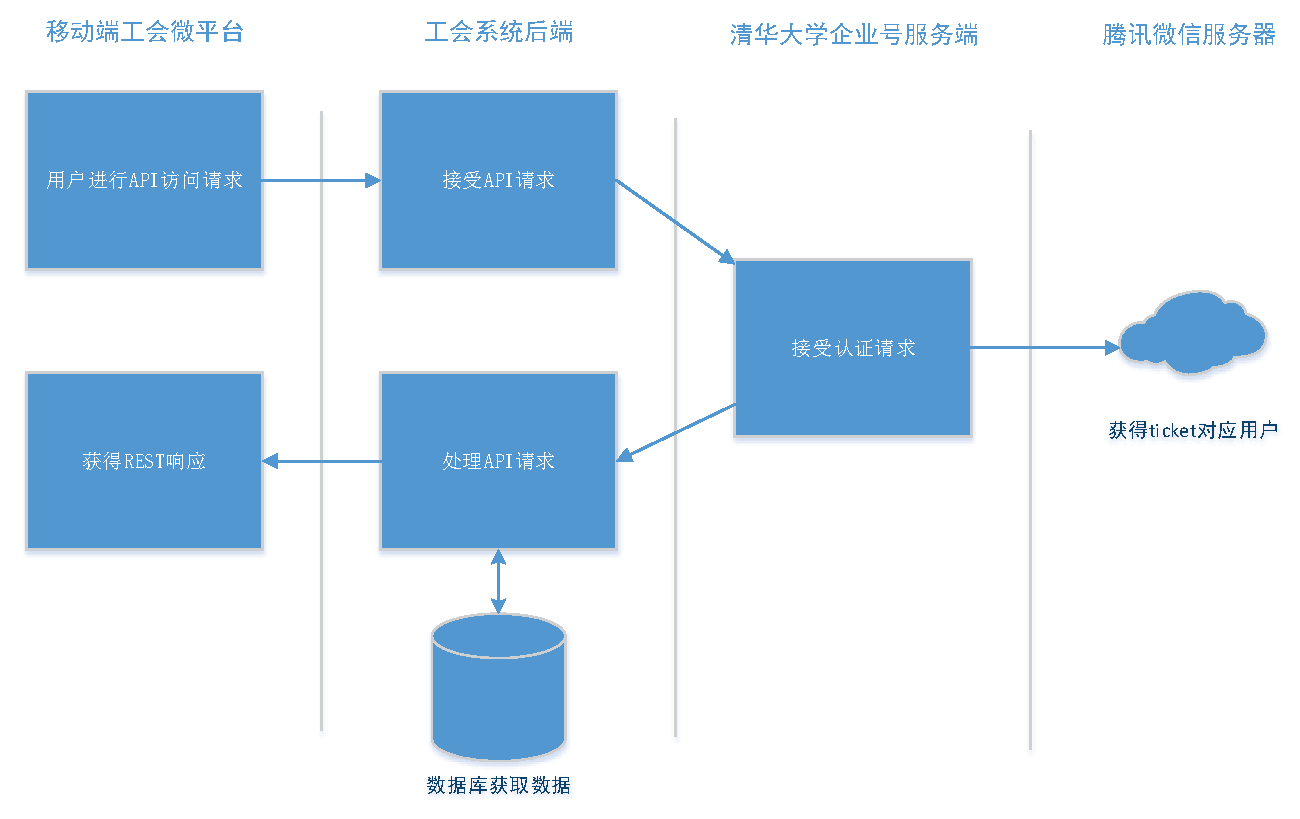
\includegraphics[width=1\textwidth]{wechatAuth}
  \caption{清华大学工会微信微平台用户认证流程}
  \label{fig:wechatAuth}
\end{figure}

通过ticket方式获得工作证号的方法避免了用户在移动设备上进行输入的繁琐,只需要其登录了微信客户端就可以通过微信认证的方式免登录地操作清华大学的工会系统了。同时这种方式也保证了用户信息的安全性,将其他的安全风险分摊到腾讯的微信服务当中去。

\section{RSA加密}

由于HTTP协议的不安全性,如果将用户名和密码等存在隐私问题的数据直接通过HTTP协议传输,那么一旦被截获就会产生密码泄露的安全问题。虽然HTTPS协议可以解决这一安全问题,但是HTTPS并不是每个服务器都可以申请进行的,绝大多数网站依然运行在HTTP协议上。

不可避免的,清华大学工会管理系统也遇到了同样的问题。系统在需要用户进行登录。在网页端进行登录的时候用户的身份验证使用的是密码。如果对密码进行可逆的加密传输,就会导致密码容易被截获并导致个人信息泄露。如果泄露的是管理员的密码信息,还会导致更严重的后果。

系统中用到的RSA认证过程如图\ref{fig:rsa}所示。

\begin{figure}[H]
  \centering
  \includegraphics[width=0.8\textwidth]{rsa}
  \caption{销毁Session的过程}
  \label{fig:rsa}
\end{figure}

为了保护使用系统的用户的信息安全,在用户进行登录行为的时候,系统后端会使用OpenSSL工具根据用户名生成一对RSA公钥私钥对,并将公钥发送到前端。前端使用jsencypt.js对密码用公钥加密,并将加密后的密码连同用户名发给后端请求验证。后端将使用RSA私钥对加密后的密码进行解密,如果解密后的结果和数据库中的密码一致,则认为登录成功,创建会话并返回结果;否则登录行为将被拒绝。

通过这种方式,用户的密码能够获得很好的保护,防止由于网络窃听而导致的密码泄露问题。
